
\documentclass[11pt,a4paper]{article}
\usepackage[utf8]{inputenc}
\usepackage{float}
\usepackage[T1]{fontenc}
\usepackage[portuguese]{babel}
\usepackage{graphicx}
\usepackage{booktabs}
\usepackage{amsmath,amssymb}
\usepackage{siunitx}
\usepackage{hyperref}
\usepackage{caption}
\usepackage{geometry}
\geometry{top=2cm,bottom=2cm,footskip=1cm}
\usepackage{xcolor}
\usepackage{sectsty}
\usepackage{subcaption}

\definecolor{navyblue}{RGB}{0, 0, 128}
\sectionfont{\color{navyblue}}
\subsectionfont{\color{navyblue}}
\subsubsectionfont{\color{navyblue}}

% --- Capa ---
\begin{document}
\thispagestyle{empty}
\begin{center}
\vspace*{2cm}

\includegraphics[width=0.4\textwidth]{logo_fct.png}\\[1cm]
{\Large \textbf{Simulação de Link de Comunicação em GNU-Radio
Testes de um recetor Low-IF (SDR)}}\\[0.6cm]
{\large CSRF -- 1º Trabalho}\\[2cm]
{\normalsize Diogo Ferreira 73076 \\ Gonçalo Dionísio 73638 \\ Iuri Moças }\\[1cm]
\vspace*{3cm}
{\normalsize Data: 25/05/2026}\\[3.5cm]
{\normalsize Departamento de Engenharia Eletrotécnica e de Computadores}\\
{\normalsize CSRF – 2026/2027 – 1º Semestre}\\
\vfill
\end{center}
\newpage

% --- Sumário ---
\tableofcontents

\listoffigures
\newpage

\section{Introdução}\paragraph{}

Este relatório descreve o trabalho laboratorial desenvolvido no âmbito da unidade curricular de Circuitos 
e Sistemas para Rádio-Frequência, centrado no estudo e teste de sistemas de comunicação por RF. 
O trabalho divide-se em três etapas principais: a simulação a nível de sistema de uma ligação de 
rádio AM com recurso ao GNU Radio; a modelação elétrica e respetiva simulação temporal e espectral 
em SPICE; e o projeto, simulação e caracterização experimental de um filtro passa-banda de 2ª ordem 
para a banda de FM com um Analisador Vetorial de Redes (VNA). Por fim, procedeu-se à integração deste 
filtro num Radio Frequency Front-End (RFFE) para montagem e teste prático de um recetor Low-IF. 
O objetivo central passa por comparar os resultados teóricos, as simulações ideais e com componentes 
reais, e as respetivas medições laboratoriais.

\section{Implementação e Simulação do Link de Comunicação em GNU Radio}\paragraph{}

A primeira parte deste trabalho foi a implementação e simulação de um link de comunicação AM 
utilizando o GNU Radio. O objetivo desta etapa foi compreender o funcionamento de um sistema 
de comunicação AM, desde a modulação até à desmodulação do sinal.

O sistema foi modelado em \textit{gnuradio-companion} com uma frequência de amostragem 
$f_s = \SI{768}{kHz}$ e uma portadora de $f_c = \SI{100}{kHz}$, dentro do intervalo 
sugerido no enunciado. O sistema é composto por um transmissor AM, um canal com ruído 
aditivo e um receptor com misturador em quadratura (IQ).

\subsection{Transmissor e canal}

A Figura~\ref{fig:tx} mostra o transmissor e o modelo do canal. A mensagem é um 
cosseno de $f_m = \SI{1}{kHz}$, multiplicado por uma constante $m$ (índice de modulação, 
$m=1$) e somado a uma constante unitária, obtendo-se o envelope

\begin{equation}
    e(t) = 1 + m\cos(2\pi f_m t).
    \label{eq:env}
\end{equation}

Este sinal é multiplicado pela portadora, resultando em AM com portadora (DSB-LC):

\begin{equation}
    s(t) = \left[1 + m\cos(2\pi f_m t)\right]\cos(2\pi f_c t).
    \label{eq:am}
\end{equation}

Expandindo~\eqref{eq:am}, o espectro apresenta a portadora a \SI{100}{kHz} e 
duas bandas laterais, a \SI{99}{kHz} e \SI{101}{kHz}, cada uma com amplitude $m/2$. 
A constante somada em~\eqref{eq:env} garante que o envelope é sempre positivo, o que 
permite a deteção de envolvente no receptor.

O canal é modelado como ruído gaussiano branco aditivo (AWGN), somado ao sinal 
$s(t)$ através de um bloco \textit{Add}. Foram incluídos \textit{QT GUI Time Sink} 
e \textit{QT GUI Frequency Sink} em vários pontos da cadeia (mensagem, sinal somado, 
sinal modulado e saída do canal) para observar a transformação do sinal.

\begin{figure}[H]
    \centering
    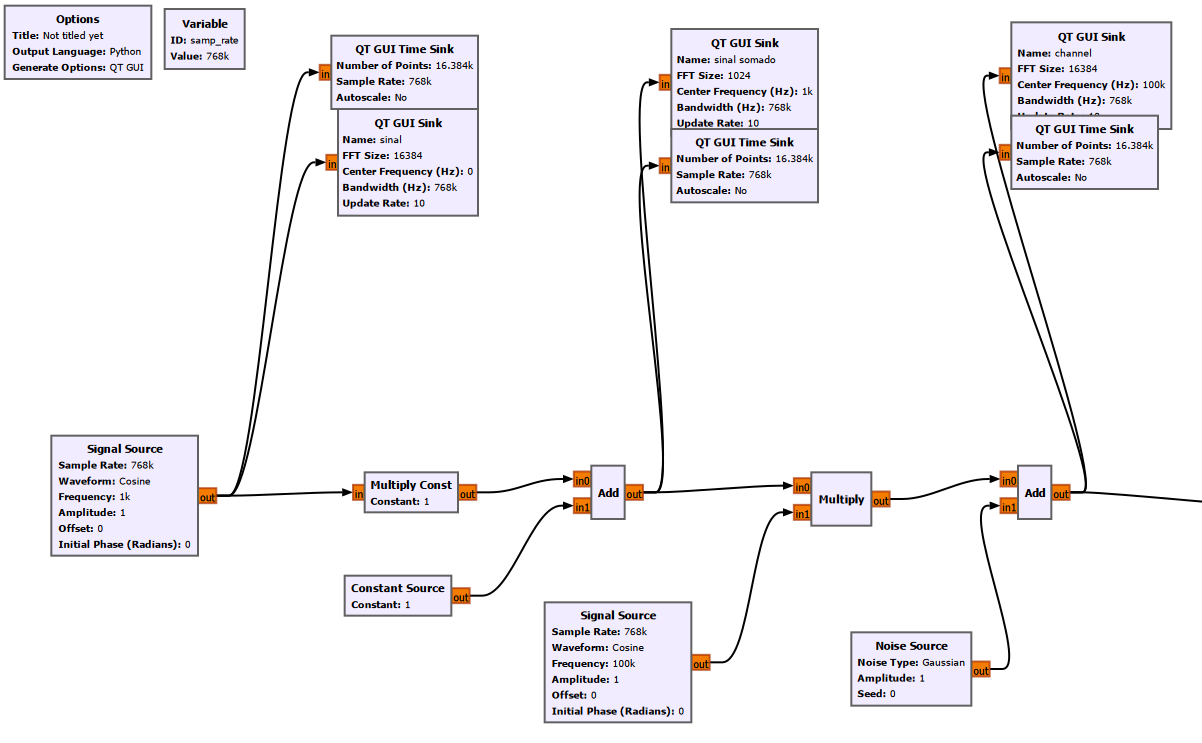
\includegraphics[width=0.9\linewidth]{GNURadio1_Cos.png}
    \caption{Transmissor AM e modelo de canal em GNU Radio: geração da mensagem, adição do \textit{offset} DC, mistura com a portadora de \SI{100}{kHz} e adição de ruído gaussiano.}
    \label{fig:tx}
\end{figure}

\subsection{Receptor}

O receptor, ilustrado na Figura~\ref{fig:rx}, implementa uma demodulação coerente com 
misturador IQ. O sinal recebido passa por um bloco de ganho ($g_1 = 1$) e é multiplicado 
por um oscilador local de \SI{100}{kHz}, em cosseno (ramo I) e em seno (ramo Q).

Cada produto contém uma componente em banda base e outra a $2f_c = \SI{200}{kHz}$:
\begin{equation}
    I(t) = s(t)\cos(2\pi f_c t) = \tfrac{1}{2}e(t) + \tfrac{1}{2}e(t)\cos(4\pi f_c t),
\end{equation}
e de forma análoga para $Q(t)$, que em banda base é nulo quando o LO está em fase 
com a portadora.

Cada ramo é filtrado por um passa-baixo (frequência de corte \SI{1}{kHz}, largura de 
transição \SI{500}{Hz}, janela de Hamming), com decimação de 16, que elimina a 
componente a \SI{200}{kHz} e reduz a taxa de amostragem para \SI{48}{kHz}, valor 
compatível com o \textit{Audio Sink}. Os ramos I e Q são combinados num sinal 
complexo (\textit{Float To Complex}) e a envolvente é obtida por
\begin{equation}
    y(t) = \sqrt{I^2(t) + Q^2(t)}.
\end{equation}
A vantagem da arquitetura IQ é que $y(t)$ não depende da fase relativa entre o 
LO e a portadora recebida: uma diferença de fase apenas redistribui a energia 
entre $I$ e $Q$, mantendo a magnitude.

\begin{figure}[H]
    \centering
    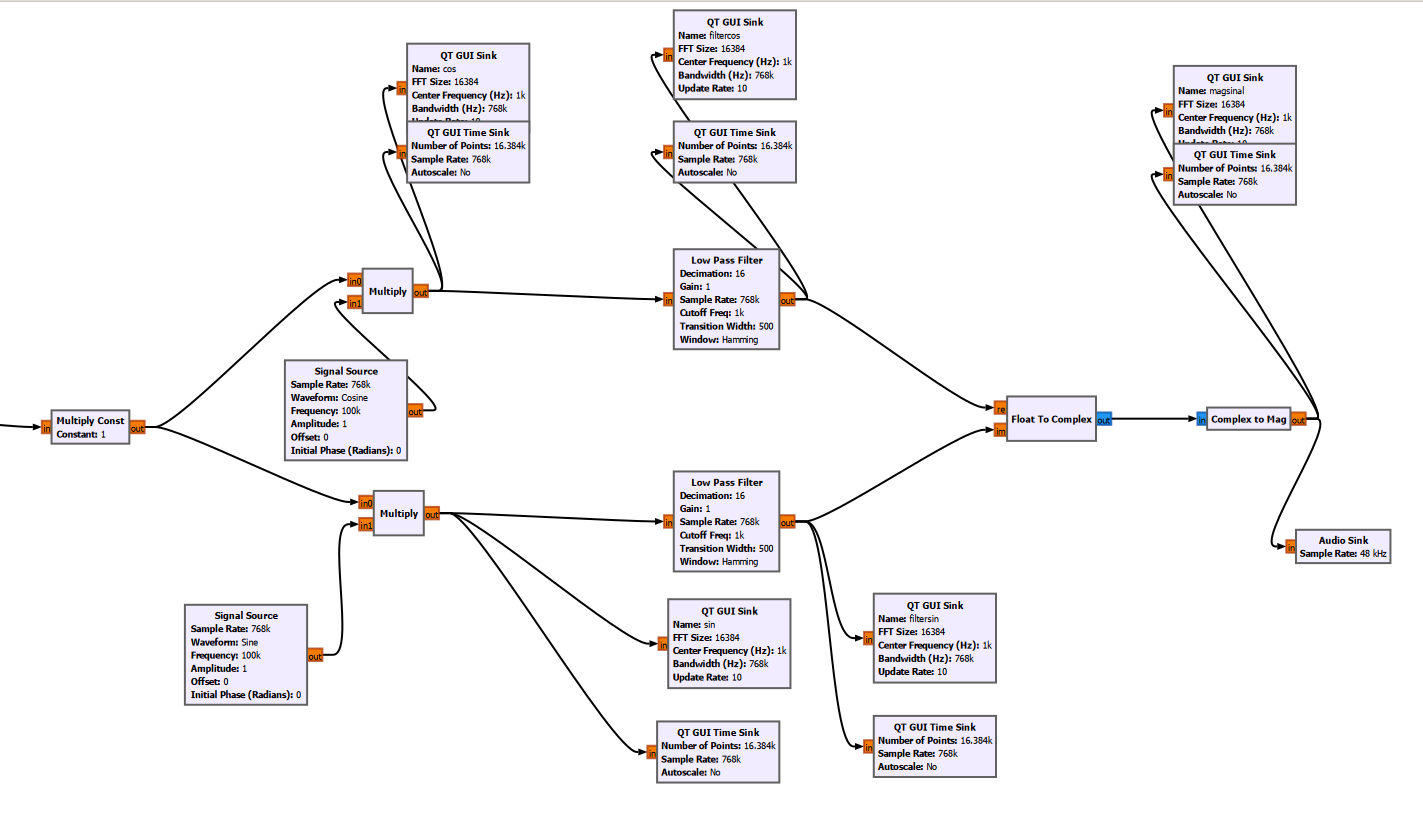
\includegraphics[width=\linewidth]{GNURadio2_Cos.png}
    \caption{Receptor AM com misturador IQ: mistura com LO em cosseno e seno, filtragem passa-baixo com decimação, combinação IQ e deteção de envolvente (\textit{Complex to Mag}).}
    \label{fig:rx}
\end{figure}

\subsection{Resultados}

A Figura~\ref{fig:tempo} apresenta os sinais no domínio do tempo e a 
Figura~\ref{fig:freq} no domínio da frequência, em pontos-chave da cadeia. 
À saída do receptor recupera-se a mensagem de \SI{1}{kHz} sobre um nível DC, 
que corresponde à portadora (termo unitário de~\eqref{eq:env}); para aplicação 
em áudio este nível pode ser removido com um bloco \textit{DC Blocker}.

\begin{figure}[H]
    \centering
    % \includegraphics[width=\linewidth]{tempo.png}
    \caption{Sinais no domínio do tempo: (a) mensagem, (b) sinal AM, (c) sinal à saída do canal, (d) saída dos filtros I/Q, (e) envolvente recuperada.}
    \label{fig:tempo}
\end{figure}

\begin{figure}[H]
    \centering
    % \includegraphics[width=\linewidth]{freq.png}
    \caption{Espectros: (a) mensagem a \SI{1}{kHz}, (b) AM com portadora e bandas laterais a \SI{99}{kHz} e \SI{101}{kHz}, (c) sinal com ruído, (d) saída dos misturadores, com componentes em banda base e a \SI{200}{kHz}, (e) saída dos filtros.}
    \label{fig:freq}
\end{figure}

\subsection{Ruído e relação sinal-ruído}

O ruído gaussiano utilizado tem amplitude 1, comparável à amplitude do sinal, 
pelo que o SNR à entrada do receptor é baixo e o ruído é claramente visível no 
domínio do tempo (Figura~\ref{fig:tempo}c). No espectro (Figura~\ref{fig:freq}c),
 o ruído distribui-se por toda a largura de banda de simulação (\SI{768}{kHz}), 
 enquanto o sinal ocupa apenas três linhas espectrais.

Os filtros passa-baixo limitam a largura de banda de ruído de aproximadamente \SI{384}{kHz} (banda de Nyquist) para cerca de \SI{1}{kHz}, o que, para ruído branco, corresponde a uma melhoria teórica do SNR de
\begin{equation}
    \Delta\mathrm{SNR} \approx 10\log_{10}\!\left(\frac{384\,\mathrm{kHz}}{1\,\mathrm{kHz}}\right) \approx \SI{26}{dB}.
\end{equation}

\subsection{Utilização de um ficheiro de áudio como mensagem}
\label{sec:wav}

Após validar o sistema com a mensagem ideal de \SI{1}{kHz}, a fonte foi substituída
por um ficheiro de áudio (\textit{.wav}, \SI{48}{ksps}). As Figuras~\ref{fig:wavtx}
e~\ref{fig:wavrx} mostram o sistema completo com as alterações.

No transmissor (Figura~\ref{fig:wavtx}), o ficheiro é lido pelo bloco
\textit{Wav File Source} e interpolado por 16 com um \textit{Rational Resampler},
passando de \SI{48}{kHz} para a taxa de simulação de \SI{768}{kHz}. O sinal é
escalado por $m = 0.5$ e somado à constante unitária, de modo a que o envelope
$1 + m\,x(t)$ se mantenha positivo para sinais normalizados a $\pm 1$,
evitando sobremodulação. A mistura com a portadora de \SI{100}{kHz} e o canal
com ruído gaussiano mantêm-se inalterados.

\begin{figure}[H]
    \centering
    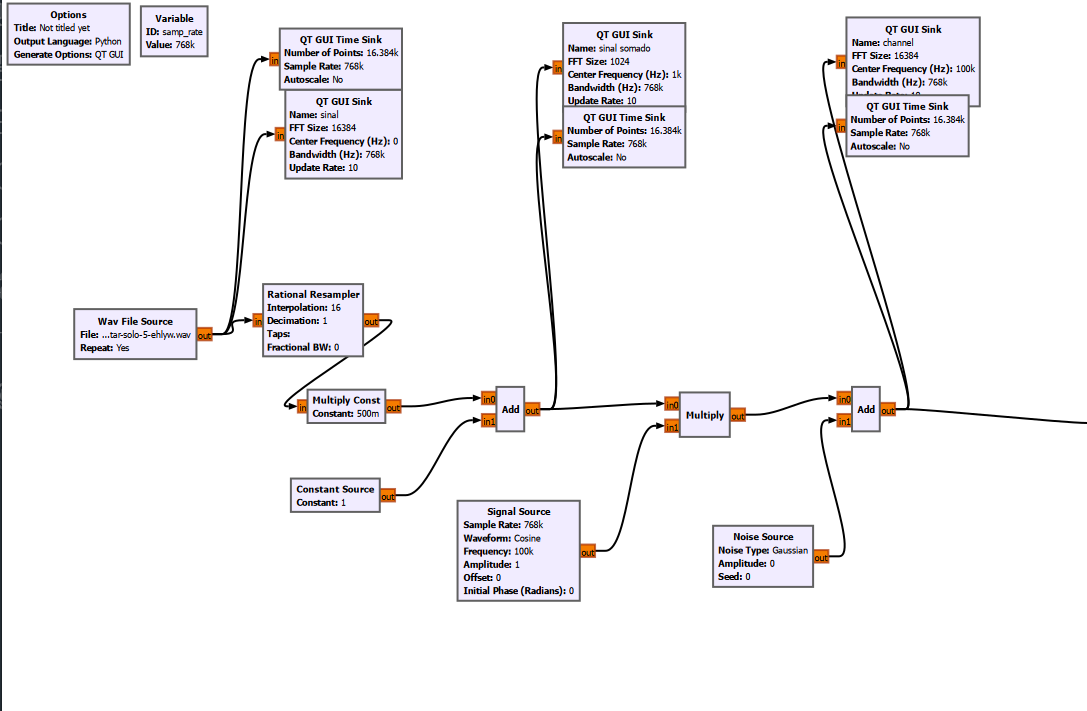
\includegraphics[width=0.9\linewidth]{GNURadio_Wav_Tx.png}
    \caption{Transmissor e canal com ficheiro de áudio como fonte: \textit{Wav File
    Source} (\SI{48}{kHz}), interpolação por 16 (\SI{768}{kHz}), índice de
    modulação $m=0.5$, adição da constante unitária, mistura com a portadora e
    ruído gaussiano.}
    \label{fig:wavtx}
\end{figure}

No receptor (Figura~\ref{fig:wavrx}), a estrutura IQ é a mesma, mas a frequência de
corte dos filtros passa-baixo foi aumentada de \SI{1}{kHz} para \SI{4}{kHz}
(largura de transição de \SI{1}{kHz}), de modo a preservar a largura de banda útil
do áudio.

\begin{figure}[H]
    \centering
    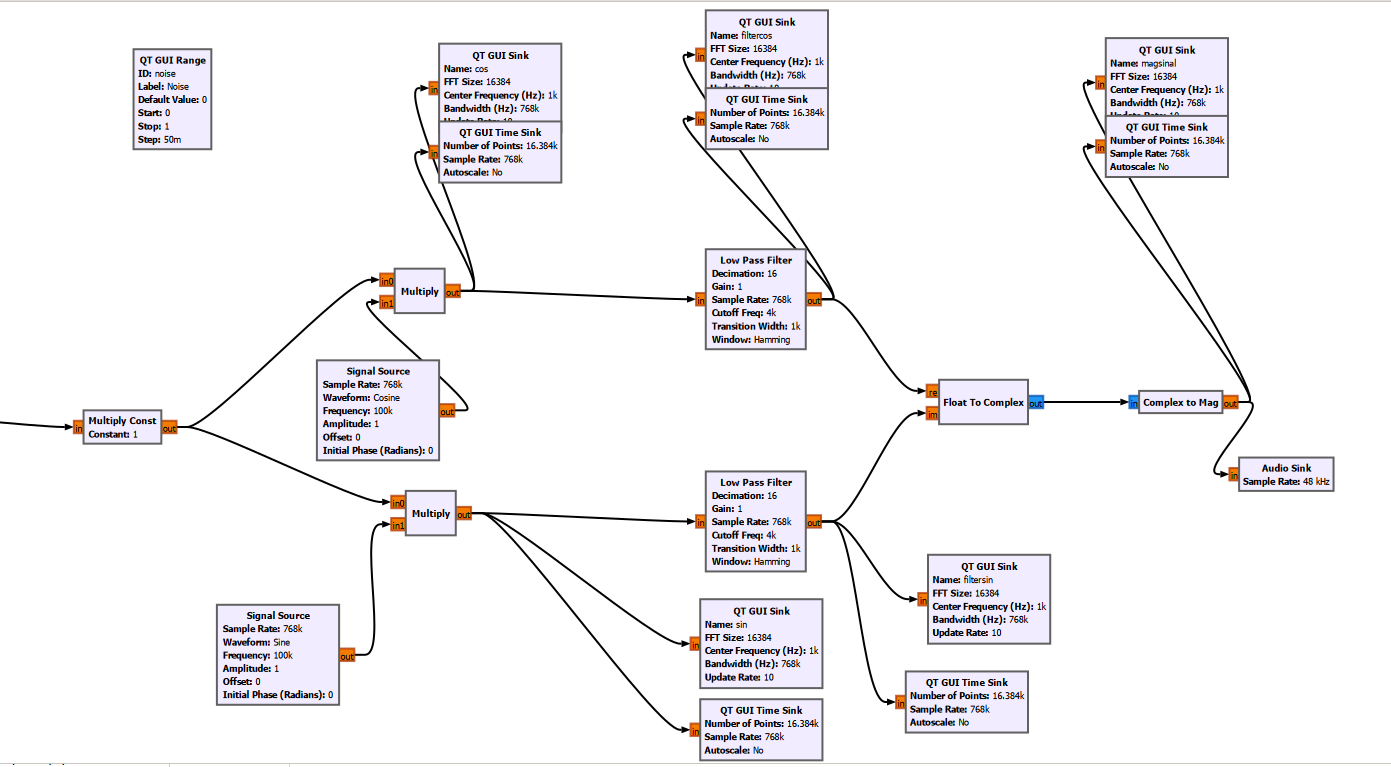
\includegraphics[width=\linewidth]{GNURadio_Wav_Rx.png}
    \caption{Receptor IQ com filtros passa-baixo a \SI{4}{kHz} e controlo do nível
    de ruído através de \textit{QT GUI Range}.}
    \label{fig:wavrx}
\end{figure}

A envolvente recuperada tem a forma $\tfrac{1}{2}\left[1 + m\,x(t)\right]$, ou seja,
um nível DC associado à portadora e um sinal útil atenuado por $m/2 = 0.25$.
Esta alteração introduz ainda um compromisso entre fidelidade e ruído: um filtro
mais largo preserva melhor o timbre do áudio, mas deixa passar mais potência de
ruído, reduzindo o SNR à saída em relação ao caso de \SI{1}{kHz}.




\end{document}
